\documentclass[a4]{article}
\usepackage{gnuplottex}
\usepackage{csvsimple}
\usepackage{subcaption}
\usepackage{amsmath}
\usepackage{graphicx}
\usepackage{epstopdf}
\usepackage{float}

\graphicspath{ {./test_data/} }

\title{COMP26120 Lab 5 Report}
\author{Ziyi Li}
\begin{document}
\maketitle


\section{What makes a problem hard for Dynamic Programming?}
Written with assistance from chatGPT

\subsection{Hypothesis}

When using a dynamic programming algorithm to solve the knapsack problem, there should be a positive relation between the backpack's size and the program's runtime, when the input data size is fixed. This means that the program takes more time to process when the knapsack size increases.

\subsection{Design}

The input data is generated by script provided (kp\_generate.py), in multiple groups. For the same size of backpack but different input data, I will run 3 groups of data with same backpack size. I hope the result will not variant. The range of size is between 1000 to 10000 with spacing 500. The the input data size(number of items) is fixed to 5000. The programs used here are dp\_kp.py and greedy\_kp.py. In order to ensure that the output does not affect the running time of the program, all outputs are turned off. Python Jupyter Notebook is used here to run test and collect data.

\subsection{Results}
\begin{figure}[H]
    \begin{minipage}{0.48\textwidth}
    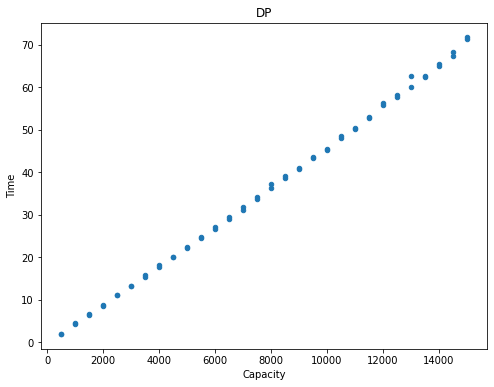
\includegraphics[width=0.95\textwidth]{dp.png}
    \caption{Dynamic Programming}
    \end{minipage}
    \begin{minipage}{0.48\textwidth}
    \includegraphics[width=0.95\textwidth]{greedy.png}
    \caption{Greedy}
    \end{minipage}
\end{figure}


\subsection{Discussion}

In the experimental data obtained by the greedy algorithm, there are a few points that do not conform to the trend, and they can be considered as errors. According to the experimental results, we can observe a direct proportionality between the knapsack capacity and the runtime of the program. This means that as the knapsack capacity increases, the program's running time also increases proportionally. This is due to the amount of data that the program needs to process also increasing, so more time is required to calculate the solution.\\

\noindent This shows that the hypothesis holds. Therefore we can conclude that the larger knapsack size makes the knapsack problem more difficult to solve.\\

\noindent In addition, the results of the greedy algorithm indicate that the running time is much smaller than that of the dynamic programming algorithm. This can be attributed to the fact that the greedy algorithm makes locally optimal choices at each step without looking ahead, and thus has a lower time complexity than the dynamic programming algorithm. While the greedy algorithm may not always produce the globally optimal solution(or correct solution), it can be a more efficient alternative to dynamic programming in so me cases, especially when the problem has a specific structure that allows for greedy choices.

\subsection{Data Statement}
All files mention below are located in test\_data folder.\\

\noindent Experiment scripts are test\_dp.py and test\_greedy.py. The scripts will use os.system to run the algorithm file, and store the runtime to pandas DataFrame, the results for both dynamic programming and greedy are in result\_dp.csv and result\_greedy.csv.\\

\subsection{Appendix}

I do give permission for this report to be anonymised and circulated within the University of Manchester to allow staff to better understand how chatGPT can be used in coursework.  I do give permission for anonymous excerpts from my report to be quoted in reports or papers about the use of chatGPT in coursework.

%% Any raw data or code scripts you want to present should be included as appendices.
\end{document}